
\documentclass[12pt]{article}
\usepackage{geometry} % see geometry.pdf on how to lay out the page. There's lots.
\usepackage{hyperref}
\usepackage{graphicx}
\usepackage{gensymb}

\geometry{letter} % or letter or a5paper or ... etc
% \geometry{landscape} % rotated page geometry

% See the ``Article customise'' template for come common customisations

\title{Gluss = Slug + Truss}
\author{Robert L. Read}

\date{\today}

%%% BEGIN DOCUMENT
\begin{document}

\maketitle

%%% Probably will want to remvoe this as the article will not be that long

\tableofcontents

\section{Introduction}

\subsection{Motivation}

Imagine a strong, light, metamorphic robotic substance.
The uses of such a substance are limited only by our ability to imagine them.

Imagine a bridge that crawls into place in a matter of hours.
Imagine constructing a temporary highway overpass in 24 hours, or a pedestrian bridge for a festival
in the morning that comes down in the evening.

Imagine a snake-like robot that can crawl into a collapsed building and hold the roof up
while survivors are extracted.
Imagine material that combines the functionality of forklift, a crane, a bulldozer and a backhoe,
all in one machine. Imagine a very small gluss that crawl into and holds shut a wound,
temporarily taking the place of missing tissue.

\subsection{Concept: Gluss = Slug + Truss}

Imagine a metamorphic machine that forcefully assumes a variety of shapes. It moves like a mollusc or amoeba,
oozing into position as commanded. It is technically a ``machine'' because it can exert force reliably, but
it may be thought of as a material, because unlike most robots its compoents are not differentiated.

Although someday an actual chemical substance may do this, today it can be constructed from commercial components
and 3D-printable parts. This paper introduces the \emph{gluss} approach to building metamorphic dynamic robots
and static machines.\footnote{ ``Gluss'' is a portmaneau of ``Slug'' and ``Truss'' because we are attempting to
build a truss, or space frame, that is capable of moving like a slug, or octopus if you prefer.
The word \textit{gluss}
should be used as a substantive noun in English, much like the word \textit{clay} is used.
The use of \textit{glusses} the plural
of \textit{gluss} should be rare and refer to different kinds of metamorphic material, such as the expression
``four clays'' suggests four distinct types of clay without specifying how many kilograms of each one means.}

Massively scalable robots have often been proposed. Our particular approach is to use linear actuators,
which are rod-like machines that can make themselves shorter or longer. These are tied together using
a relatively new joint \cite{song2003spherical} which allows, for example, as many as 12, but more realistically 4,
members to be joined together sturdily at a single point.
A 3-D printed embodiment presented here and called the \emph{turret joint} to allow the
change of angle to allow gluss to ooze about. Some gluss consists of some actuators joined together
with some turret joints and whatever batteries and control microelectronics are needed. In the
working, crawling robot discussed here, the \emph{3TetGlussBot}, there are two controllers and two batteries
in addition to the 12 actuators and the 6 multi-member turret joints, but 3TetGlussBot is only
a small amount of the gluss we hope to build.

\begin{figure}[!ht]
  \centering
    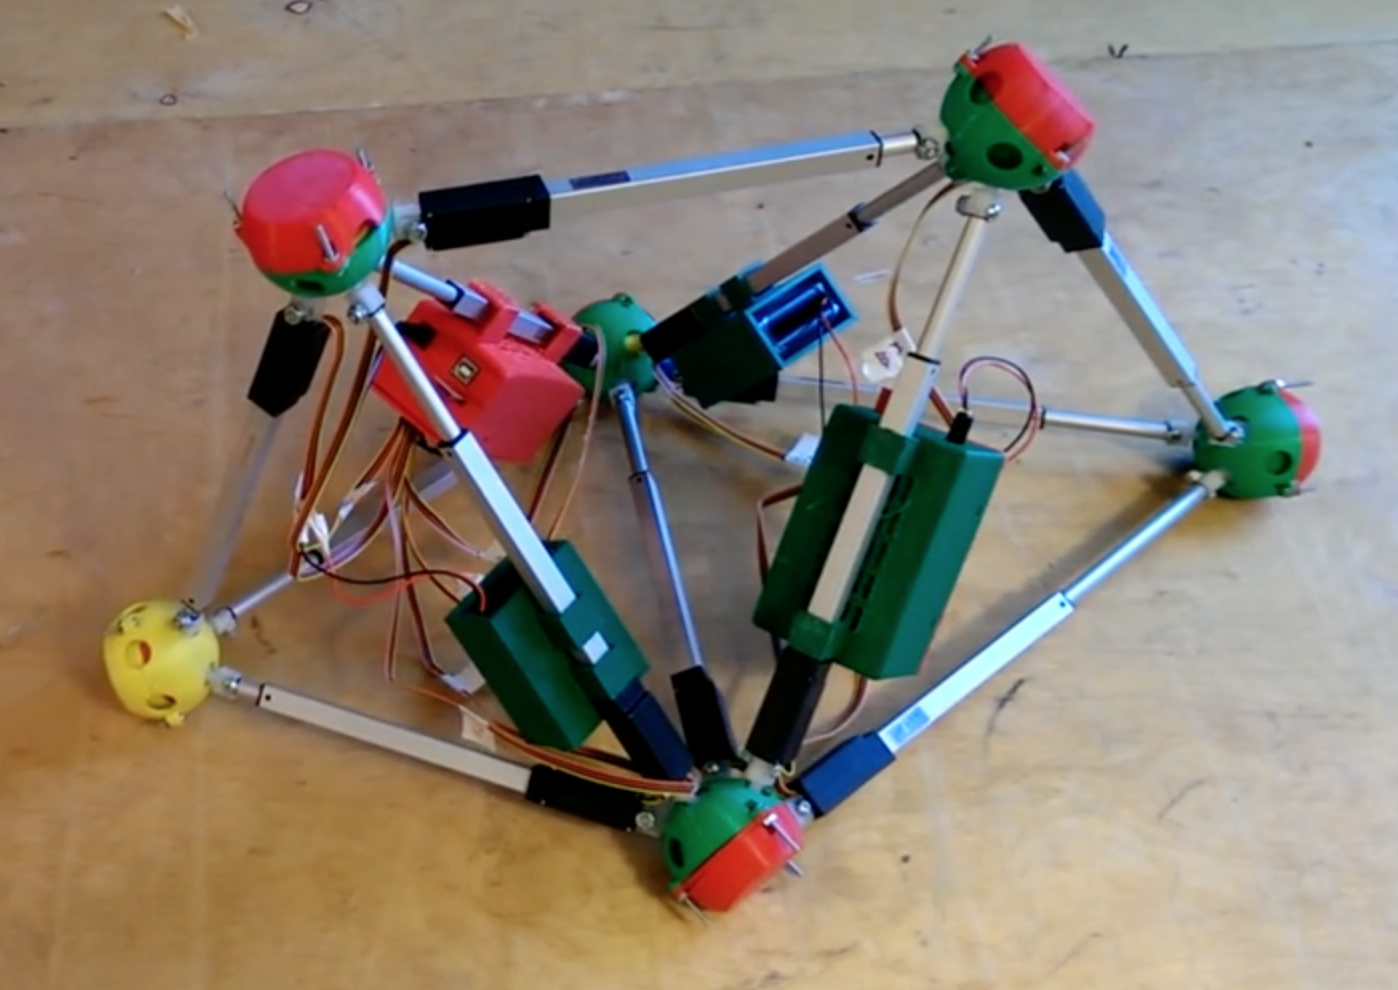
\includegraphics[width=0.5\textwidth]{3TetGlussBotPhoto.png}
    \caption[3TetGlussBot Photo]{Photo of the 3TetGlussBot.}
      \label{3TetGlussBotPhoto}
\end{figure}


We present two geometries for gluss which have the advantage of being regular, thus allowing us to
seamlessly connect any number of actuators into any amount of gluss.
The specific actuators, their 12 Volt power supply, control via Arduino Mega microcontrollers, and
coordination via BlueTooh from an Emacs E-LISP control program are discussed.

\section{The Turret Joint}

\subsection{The Need}

The way to make some thing large, light, and strong is to make it inherently rigid by building it
out of triangles. In a single plane, this is called a \emph{truss}, and more generally is called
a \emph{space frame}.  Space frames made completely from triangles tend to be rigid even if the
joints that connect members are allow motion, such as a pin joint or a ball-and-socket joint. This
is an advantage because strain (that is, a slight change in the geometry of the frame) cannot cause
the joint to fail, as it can with a welded joint.

But we seek a space frame that can change its shape dramatically. Imagine a radio tower in which
each girder has been replaced with an actuator that can get longer or shorter. Such a tower could
bend its top down to the ground, or event
tie itself into a knot. To accomplish this, the joints must support significant although not
limitless range of motion. 

The spherical joint inveted by Song, Kwon and Kim \cite{song2003spherical} is such a joint.
In the embodiment mentioned here joint presented here supports somewhat less than a theoretical
$36\degree$ of motion.
When properly configured to support the regulat nets of actuators we propose,
it allows the gluss to be a moving spaceframe. It happens that the specific actuators we use
are geared such that they hold their position forcefully without power, so the resulting gluss
can move into position and then be powered off to be a temporarily static space frame.

One could also use this joint with members which are not actuators. For example, we first
constructed the joint with carbon fiber rods. In essence it is then becomes a construction with continuously
variable member lengths liberated from using a finite set of angles.

\subsection{The Turrent Joint}


\begin{figure}[!ht]
  \centering
    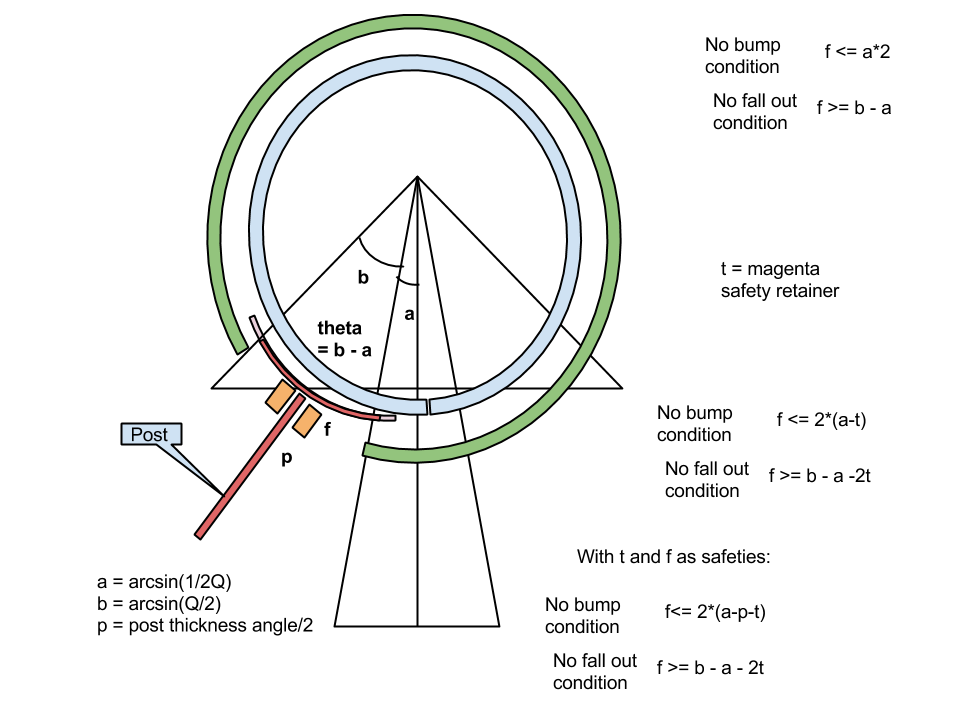
\includegraphics[width=0.5\textwidth]{TurretJointMath.png}
    \caption[TurretJointMath]{The Turret Joint analyzing the range of motion. TODO: This needs to be improved, showing the golden triangle and golden gnomon!}
      \label{TurretJointMath}
\end{figure}


\subsection{Embodiment}

\subsection{Geometries Specific to Gluss}

Although the possibly ways to configure acutators and joints is limitless, the simplest thing is to
use regular, repeatable geometries. The two most obvious are the Boerdijk–Coxeter helix
(more easily called the \textit{tetrahelix}) \url{https://en.wikipedia.org/wiki/Boerdijk%E2%80%93Coxeter_helix}
  (See Figure \ref{Boedijk-Coxeter-Helix}) and the \emph{Octet Truss} \cite{richard1961synergetic} (See Figure \ref{octet-truss-patent}).
Roughly speaking, the Tetrahelix is a good way to make a long shaft or tentacle, and the octet truss
is a good way to make a planar shape. The purpose of a tentacle is to curl, and the we have no word for
a plane that roll itself up into a cylinder or cone or form a barrel vault.


\begin{figure}[!ht]
  \centering
    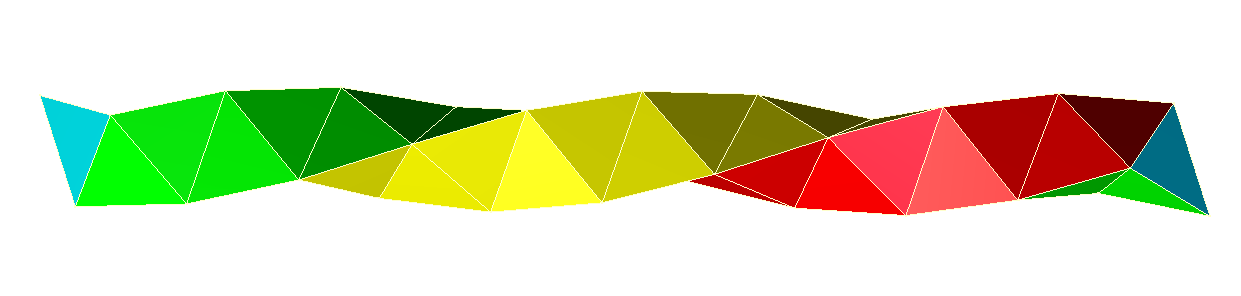
\includegraphics[width=0.5\textwidth]{Coxeter_helix_3_colors_cw.png}
    \caption[Boerdijk–Coxeter Helix]{Boerdijk–Coxeter Helix, or Tetrahelix, By Tomruen (Own work)
      [CC BY-SA 4.0 (\url{http://creativecommons.org/licenses/by-sa/4.0})], via Wikimedia Commons}
      \label{Boedijk-Coxeter-Helix}
\end{figure}

\begin{figure}[!ht]
  \centering
    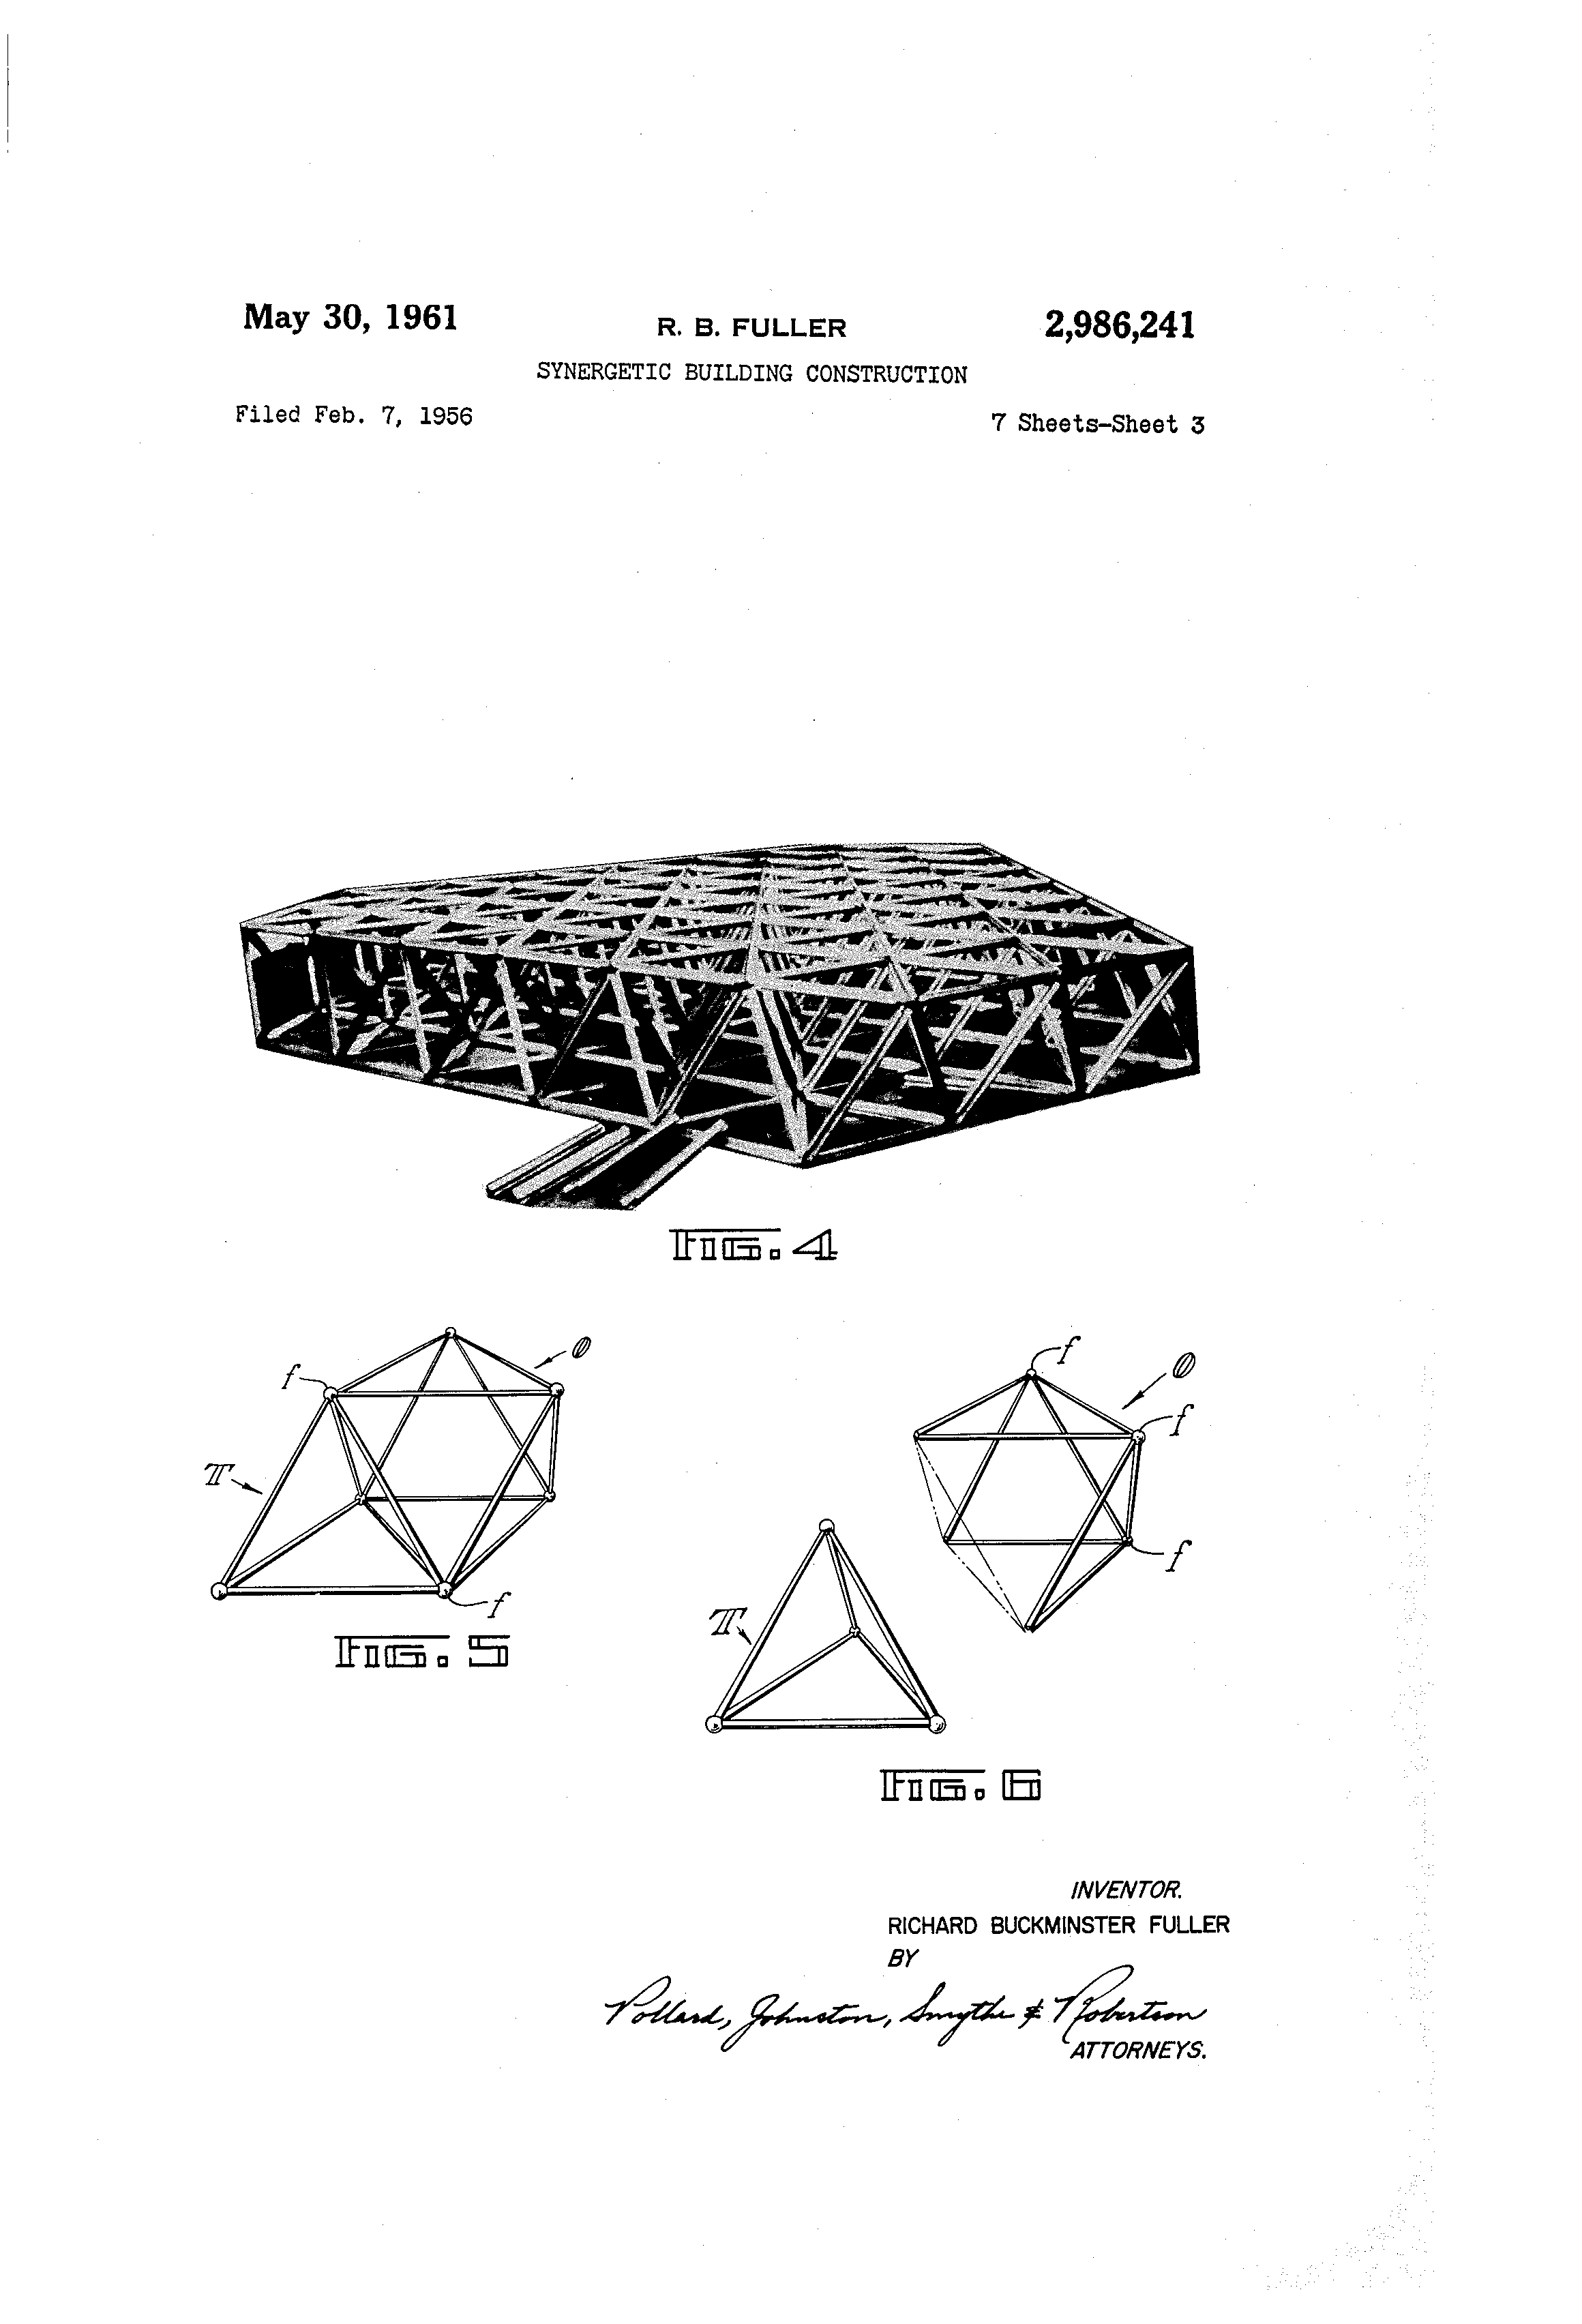
\includegraphics[width=0.5\textwidth]{US2986241-2.png}
    \caption[The Octet Truss]{The Octet Truss, from Buckminster Fuller's patent.}
      \label{octet-truss-patent}
\end{figure}

\subsection{Range of Motion for Actuator Nets}

Put the math here.

\section{Linear Actuators}

We use the term Linear Actuator to refer to any device that is capable of changing its length. When
used in gluss it might be called a \emph{glussion}, a single particle of gluss. Our current gluss
uses a commercial linear actuator (the Firgelli L-16-140-35-12-P, \url{http://www.firgelli.com/L16_Linear_Actuators_p/l16-p.htm}) that costs about \$80 and exerts about 50 Newtons of force.
Turret joints that are 3D printed in ABS plastic have been strong enough for this level of force.

However, in principle there is not reason we could not use the enormous hydraulic cylinders
used backhoes, bulldozers, and other earth moving equipment. These would of course require much
stronger joints, probably not made out of plastic.

We could also attempt to make smaller actuators, to make a pocket-sized gluss. This is probably
a greater technical challenge, because it is relatively difficult to make small electric motors.

The current actuators use a rotary motor with a lead screw. This has the advantage of great
strength relative to their size, and the retaining position forcefully. It has the disadvantage
of being relatively slow. It would be interesitng to build a gluss out of linear motors, for
example tubular linear synchronous motors. These would be much faster than the lead-screw type
actuators, resulting in a much faster gluss. 

\section{Control and Motion}
\subsection{Architecture of the 3TetGlussBot}

We have constructed the simplest possible Tetrahelix-based glussbot that is capable of locomotion.
It comprises:
\begin{itemize}  
\item 12 actuators
\item 6 turret joints
\item 2 12V battery packs
\item 2 controller units, each of which comprises:
\begin{itemize}  
\item 1 Arduino Mega microcontroller,
\item 1 custom Arduino Mega shield hosting 6 1-amp motor channels and a BlueTooth module,
\end{itemize}  
\end{itemize}

[TODO: a diagram with pointers here.]

Each controller module electrical system can support up to 6 actuators, so two are required for the 3TetGlussBot.
The BlueTooth modules open serial connections controlled by a computer.
The Arduino Mega is programmed to support commands addressed to each or all of the actuators, and
to provide feedback. The comptuer and the Arduino control programs communicate via S-Expressions
implemented with our own module. This is very analagous to sending JSON back and forth.

Commands to and feedback from the controller modules are managed by an Emacs E-Lisp program.
This program organizes motion into ``poses''. A serious of poses make a dance.
In order to dance, the program must synchronize the completion of poses, because there is no
guarantee how long it will take to achieve a pose. The time to reach a position in theory
depends on the voltage level provided by the battery and the force resisting the motion.
In practice, when lightly loaded by moving only itself, the time is relatively predictable. It takes
about 2 seconds for the 3TetGlussBot to go from its most compact state to its largest, most expanded state.

\subsection{Open Source Realizations}

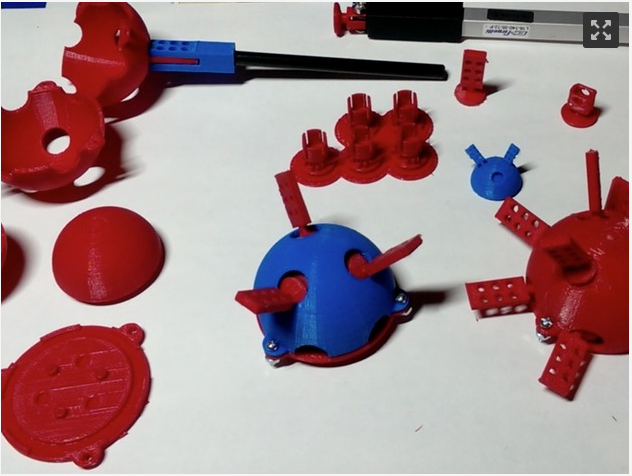
\includegraphics[scale=0.5]{TurretJointPieces.png}

\subsection{Speed Performance}

The 3TetGlussBot is capable of ``walking'' and turning. Some might prefer the term ``crawl'' to ``walk'' in
this case. It can move forward awkwardly at a rate
of about five inches per minute. It can turn 30 degrees in about 20 seconds [TODO -- need to check this.]
We intentionally chose to make the simplest amount of gluss that we thought would be capable of locomtion.
We believe that by adding more gluss, that is, by connectiong more tetrahedra in the tetrahelix,
we will open new and more efficient locomotion gaits.

The present mode of walking avoids dragging the pseudopods by leaning to one side or front or back and
then lifting the pseudopod, moving it forward (without ground contact), and placing it down again.
Such a gait may be able to handle rugose terrain better than a gait that drags feet.

The current programmed gaits are probably not optimal.
We have programmed locomotion of the 3TetGlussBot only to prove that it can be done, not to make
a performant robot.

\subsection{Force Performance}

It would be be nice to answer the questions such as:
\begin{itemize}  
\item If a 5-tetrahedron tetrahelix were bolted to a frame and extended horizontally, how much
  weight can it support at the free end?
\item If a gluss bot crawled under a car and sought to jack up the car enough for a tire
  to be changed, how forceful would each actuator have to be?
\item If a large glussbot crawled across a chasm, could a truck or a human being safely move
  across it without danger of collapse?
\end{itemize}

We have not attempted to analyze gluss in terms of force performance. We believe this would
be analagous to analysis of static space frames using the dynamic configuration at a point.
Finite elment analysis is a standard approach to this.

\section{Future Steps}

Actions are available at the research level and at the hobbyist level, and we refuse to draw
a crisp distinction betwen the two, but we have organized these from most difficult to least
difficult.

\begin{description}
\item [Remove Scale] At present the 3TetGlussBot is programmed as specific geometry. Any program
  written for it would have zero valua for a robot of the same general shape but built with considerably
  more actuators. Ideally, we would be able to program gluss completely independent of the scale
  of implementation. We would treat it as a true metamorphic material, rather than as a net of
  actuators arranged in a particular configuration. This can be considered a problem of pure
  mathematics, touching on wavelet theory, for example. It blends into computer science and
  finally robotics.
\item [Cheap Actuator] The gluss concepcts heightens the need for very inexpensive linear
  actuators. The current actuators at \$80 make construcitng a 100-actuator glussbot very expensive.
  It should be possible to build a linear actuator for 1/10th of this cost, although it may require
  giving up some advantages. Creating a new point in the spectrum of actuators desings would greatly
  expand the possibilities of gluss.
\item [Applications] A killer application would help motivate the gluss concept. This does not
  require engineering, but requires careful thought.
\item [Quick Joint] If all of the turret joints in the 3TetGlussBot are dissassembled so that
  the linear actators can be stacked together for efficient transport, it takes more than an hour
  to bolt them back together. It would be very convenient to have a joint that could be
  disassembled and assembled more quickly. We suspect that it is possible to build a magnetic
  joint similar (but larger) than those used in the GeoMag toy.
\item [Build Simulator] A 3TetGlussBot can be constructed for about \$1300. Nonetheless this
  is beyond the means of many hobbyist. A simulator would allow one to research locomotion and
  motion without cost. The open-source, browser deliverable physics engine ``Cannon.js''
  provides all the basic machinery needed to build such a simulator.
\item [Force Performance] A simulator could be extended to provide a force analysis of configurations.
  
  
\end{description}

\bibliographystyle{IEEEtran}
\bibliography{IEEEabrv,gluss}

% \bibliography{gluss}{}
% \bibliographystyle{acm}


\end{document}
